\subsection{Assurance claims for quasi synchronous systems}

Synchronous models are easier to understand give more assurance properties, but keeping a distributed system synchronized is expensive in terms of computing time and exchanged messages, which leads to less efficient implementations.
Recent work proposes a method to translate a synchronous model to an equivalent Loosely Time-Triggered Architecture where nodes communicate through FIFOs with size 1 or 2 (see \cite{LTTA}).

However, a Finite FIFO Platform assumes the nodes skips a step when its output buffers are full. Used with a ROS architecture, this model is really vulnerable to attacks.
Assume an attacker compromised a node or created a useless one; then, by subscribing to many topics but refusing to read anything (to free space in the queues), it would cause the whole system to stop working.
Moreover, these proofs assume the communication channels preserves the order of messages, which is not necessarily the case in ROS.

\paragraph{ } The other approach is to prove properties directly for the quasi synchronous system, in order to use them for more complex applications. 
Then, such properties can be used for example to map synchronous arguments to quasi-synchronous systems (see \cite{Caspi}).
This work also describes a voting procedure in this case that asserts fault tolerance; that is, providing correct inputs even with faulty sensors.

Again, some assumptions are made that are few compatible with HACMS requirements. Considering that components have a periodic execution (with a period only known to be between some bounds) takes account of local clock uncertainty.
This is sufficient when the execution rate is reasonably slow, but with a higher rate, scheduling effects and variable computation time (depending on the input) should also be considered.
Also, while direct bus communication or shared memory ensure a message is available almost as soon as it is written, safety procedures in the underlying mailbox system in HACMS makes the transmission delay non negligible.



\subsection{Security and reliability in HACMS}

As part of the HACMS project, a \emph{Robot Architecture Description Language (RADL)} is being developed.
This language is used to describe the systems functional structure, that is nodes and topics are declared with their characteristics: rate, published and subscribed topics for nodes, message type for topics (see Figure~\ref{RADL}).
This allows two different tasks:

\begin{itemize}
\item checking architecture consistency: for example, message types must match for a topic and nodes publishing or subscribing to this topic.
This also allows to check various physical requirements. Among others: a physical device can be assigned to at most one node, or at most one node is allowed to publish on a given topic.

\item generating the running ROS configuration: ROS configuration files are automatically generated from the RADL according to the specified architecture.
A portion of node running code is also automatically generated. This includes initialization steps, and the few commands to read and check incoming messages at each periodic step.
The user has to write the so called \emph{step function}, that writes messages to published topics according to input values passed as arguments.
\end{itemize}

\begin{figure}[ht]
\begin{center}
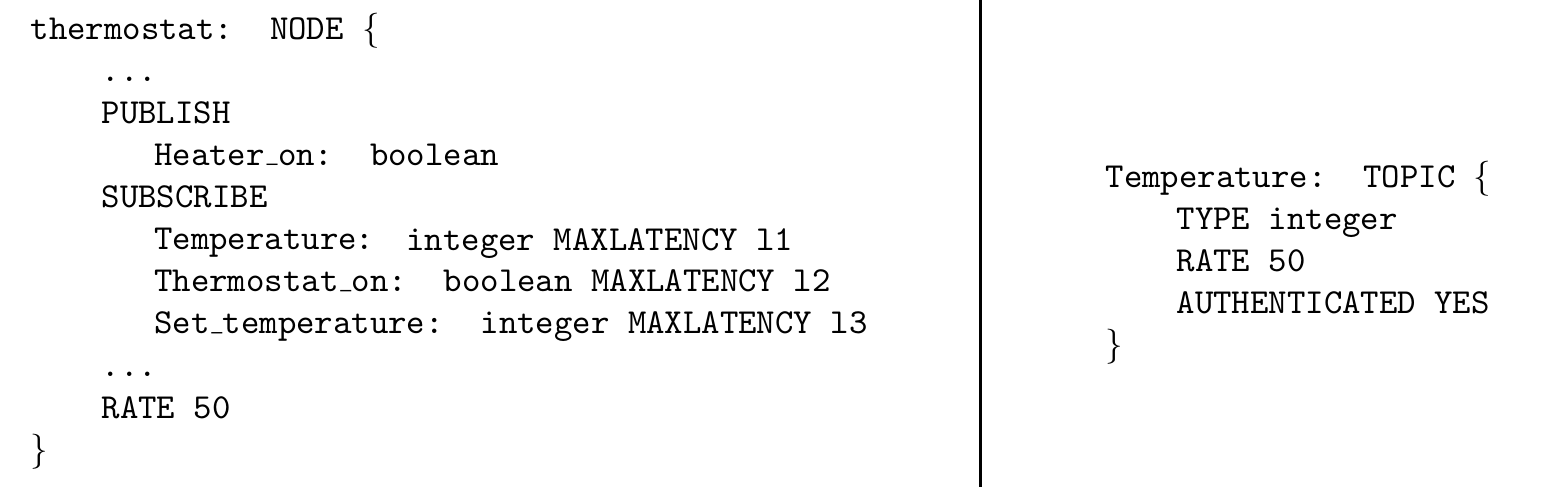
\includegraphics[width=15cm]{RADL.png}
\caption{A small RADL example}\label{RADL}
\end{center}
\end{figure}

Another interest is that the assurance properties from Section~\ref{prop} could be integrated to the code generated from RADL:
automatic checks could be added when reading input buffers, and when a node detects a behavior outside the framework given by these properties, it can report this error to a monitor and/or add a flag to sent messages to inform other affected nodes of this issue.
This allows attack detection as well as monitoring for software or hardware failure.

\paragraph{ }
Establishing assurance properties for a cyber-physical system means ensuring its behavior responds to the specification, even in presence of an attacker, and the HACMS project led to interesting work in this domain.

Security protocols and cryptography aren't enough to avoid a cyber-physical system being attacked: physical components can also being compromised.
An attacker can modify the physical environment around a sensor in order to inject malicious signal and to modify the system behavior.
A team from the University of Pennsylvania designed an algorithm to prevent such attacks (see \cite{StateEstimator}).
This algorithm ensures the state estimation error is bounded as soon as less than half the sensors are under attack (other sensors may experience a bounded noise).

This team also developed a cruise controller (see \cite{CruiseControl}) to control the speed of a vehicle. 
It ensures the difference between desired speed and actual speed is bounded after some time $T$, and this difference is exponentially decaying from time 0 to T.
The combination of the attack-resilient state estimator and the cruise controller ensures the vehicle travels at the speed set by the operator even when some sensors are compromised.



\subsection{The Prototype Verification System}

The \emph{Prototype Verification System (PVS)} is a specification language and theorem prover. The specification language uses typed higher-order logic.
Typing is needed to keep higher-order logic consistent, and also help to detect errors in the specification.
For instance, when the typechecker encounters an expression of the form \texttt{x/y}, it generates a \emph{Type Correctness Condition (TCC)}, that is a proof obligation to ensure \texttt{y} cannot be 0 in the current context.
Most of the time, automatic decision procedures manage to prove such TCCs, but sometimes, a user-made proof needs to be done\footnote{$ $
the rich type system in PVS, including constrained as well as uninterpreted subtyping, makes it non algorithmically decidable}
(and sometimes, the generated TCC is unprovable because of an error in the specification).
A more complete description of PVS can be found in the PVS user guide \cite{PVS:userguide}.

\begin{table}[ht]
\begin{center}
\begin{tabular}{|c||c|c|}
\hline
& \textbf{left} & \textbf{right} \\ \hline \hline
Axiom & 
\multicolumn{2}{|c|}{
\cell{\overline{\Gamma , A \vdash A , \Delta}}} \\ \hline

Bool. const. &
\cell{\overline{\Gamma , \texttt{FALSE} \vdash \Delta}}&
\cell{\overline{\Gamma \vdash \texttt{TRUE}, \Delta}} \\ \hline

Cut & 
\multicolumn{2}{|c|}{
\cell{\frac{\Gamma , A \vdash \Delta \qquad \Gamma \vdash A, \Delta}  {\Gamma \vdash \Delta }}} \\ \hline

$\neg$ &
\cell{\frac{\Gamma , \neg A \vdash \Delta}{\Gamma \vdash A , \Delta}}&
\cell{\frac{\Gamma \vdash \neg A , \Delta}{\Gamma , A \vdash \Delta}}\\ \hline

$\vee$ &
\cell{\frac{\Gamma , A \vdash \Delta \qquad \Gamma , B \vdash \Delta}  {\Gamma , A \vee B \vdash \Delta }}&
\cell{\frac{\Gamma \vdash A, B \Delta}  {\Gamma \vdash A \vee B, \Delta }} \\ \hline

$\wedge$ &
\cell{\frac{\Gamma , A, B \vdash \Delta}  {\Gamma, A \wedge B \vdash \Delta }}&
\cell{\frac{\Gamma \vdash A, \Delta \qquad \Gamma \vdash B, \Delta}  {\Gamma \vdash A \wedge B \Delta }} \\ \hline

$\implies$ &
\cell{\frac{\Gamma \vdash A, \Delta \qquad \Gamma , B \vdash \Delta}  {\Gamma , A \implies B \vdash \Delta }}&
\cell{\frac{\Gamma , A \vdash B \Delta}  {\Gamma \vdash A \implies B, \Delta }} \\ \hline

$\exists \: ^*$ &
\cell{\frac{\Gamma , A[\mathbf{x'}/x] \vdash \Delta }{\Gamma , \exists x . A \vdash \Delta}} &
\cell{\frac{\Gamma \vdash \Delta , A[\mathbf{t}/x]}{\Gamma \vdash \Delta , \exists x . A}} \\ \hline

$\forall \: ^*$ &
\cell{\frac{\Gamma, A[\mathbf{t}/x] \vdash \Delta}{\Gamma , \forall x. A \vdash \Delta}} &
\cell{\frac{\Gamma \vdash \Delta , A[\mathbf{x'}/x] }{\Gamma \vdash \Delta , \forall x . A}} \\ \hline

\multicolumn{3}{c}{
\begin{minipage}{13cm}\vspace{0.1cm}
$^*$ Quantifier elimination rules assume $\mathbf{x'}$ (in $\exists$~\emph{left} and $\forall$~\emph{right}) is a free variable that has no free occurrence in the sequent formulas.
Also, $\mathbf{t}$ (in $\exists$~\emph{right} and $\forall$~\emph{left}) is a term that doesn't contain a quantified variable appearing in any sub-formula of $A$.
\end{minipage}}

\end{tabular}
\end{center}

\caption{The (main) inference rules of sequent calculus}\label{LK}

\end{table}

The theorem prover is based on the inference rules of sequent calculus for propositional logic (see Table~\ref{LK}).
The prover is highly interactive and the user can choose which inference rule use at each branch of the proof tree until said branch leads to an axiom (which is a sequent calculus demonstration).
Sets of antecedent formulas $\Gamma$ are seen as a conjunction and consequent formulas $\Delta$ as a disjunction:
\[ \Gamma \vdash \Delta \quad \textrm{means} \quad \bigwedge \Gamma \implies \bigvee \Delta \]

The complete list of prover commands is available in the PVS prover guide \cite{PVS:prover}, but we present here the most useful. The \emph{Cut} rule with formula $A$ can be applied with the \texttt{case $A$} command.
\texttt{flatten} applies all possible simplifications for \emph{$\implies$ right, $\vee$ right, $\wedge$ left} and $\neg$.
\texttt{split} applies inference rule $\implies$\emph{left}, $\vee$ \emph{left} and $\wedge$ \emph{right} on a specified formula. 
\texttt{prop} is equivalent to applying \texttt{flatten} and \texttt{split} on every formula of the sequent (that can lead to a lot of subgoals).
Finally, \texttt{skolem} and \texttt{instantiate} are the quantifier elimination commands, for $\forall$ \emph{right}/ $\exists$ \emph{left} and $\forall$ \emph{left}/ $\exists$ \emph{right} respectively.

Some other useful commands are not associated to an inference rule but are shortcuts used in natural deduction.
\texttt{assert} is a light SMT (satisfiability modulo theories) solver that deals with equality theory, can simplify algebraic expressions over $\mathbb{R}$ up to a certain point and use some specific theorems.
\texttt{lemma \emph{thm}} adds the statement of theorem \texttt{\emph{thm}} to the set of antecedent formulas and \mbox{\texttt{expand \emph{name}}} replaces \texttt{\emph{name}} by its expanded definition.
\texttt{replace} uses an antecedent formula $\mathbf{t = t'}$ (where $\mathbf{t}$ and $\mathbf{t'}$ are terms) to replace $\mathbf{t}$ by $\mathbf{t'}$ in a given formula.


\paragraph{ } All results presented in Sections 4 to 6 have been formally proved using PVS. As we will see, proofs in Sections 5 and 6 are very similar.
These PVS proofs, currently \emph{hello world} examples, could become the base for automated proof procedures for such properties.


